\documentclass[11pt,letterpaper]{article}
\usepackage{graphicx}
\usepackage{geometry}
\usepackage{amsmath}
\usepackage{amssymb}
\usepackage{hyperref}
\usepackage{url}
\usepackage{natbib}
\usepackage{booktabs}
\usepackage{xcolor}
\usepackage{listings}
\usepackage{multirow}
\usepackage{array}
\usepackage{caption}

\geometry{margin=1in}
\hypersetup{colorlinks=true, linkcolor=black, citecolor=black, urlcolor=black, pdftitle={M-IRT: Reference-Free LLM Evaluation via Samejima Graded Response Models on Dynamically Generated Metamorphic Item Clusters}, pdfauthor={Anonymous}}
\urlstyle{same}

\title{\textbf{M-IRT: Reference-Free LLM Evaluation via Samejima Graded Response Models on Dynamically Generated Metamorphic Item Clusters}}

\author{Anonymous Authors}

\date{}

\begin{document}
\maketitle

\begin{abstract}
Static LLM benchmarks with frozen held-out answer keys have become suspect as language models are trained on increasingly large fractions of the public web. We ask a sharper question: can reasoning capability be measured when no answer key is trusted to be free of contamination? We introduce Metamorphic Item Response Theory (M-IRT), a reference-free framework that scores an LLM's internal logical coherence across dynamically generated Metamorphic Item Clusters (MICs). Each cluster carries four variants (seed, paraphrase, negation, and inverse or contrapositive) bound by a relational invariant whose oracle is derivable from the question text alone, so no absolute label exists. An ordinal coherence grade per (model, cluster) cell feeds a Samejima Graded Response Model (GRM) fit by marginal maximum likelihood, recovering a per-model latent ability $\theta$ and per-item discrimination and difficulty. Across five public LLMs and 100 MICs spanning propositional syllogisms and grade-school arithmetic, the $\theta$ ranking correlates with published MMLU accuracy at Pearson $r = 0.975$ and exceeds three simpler binary consistency metrics computed on the same clusters. A stress test in which a model's seed response is forced to the oracle on 30\% of clusters confirms that coherence grading penalises internally inconsistent response profiles. The pipeline is reproducible for under \$0.05 in three minutes. The headline is methodological: the GRM scaling layer, the dynamic cluster generator, and a clearly scoped protocol for the natural-contamination experiment (system-prompt injection plus re-query) that the framework's hypothesis requires.
\end{abstract}

\section{Introduction}

Benchmarks orient AI. They specify what is worth measuring and, in doing so, shape what is worth improving \citep{Liang2022}. For language models, this role has been carried by fixed, curated test sets: a frozen set of items with a frozen answer key, run against a frozen evaluation harness. HELM argued that the field needed broader coverage and multi-metric measurement, not that the frozen-test-set axiom itself was at risk. Six years on, that axiom is breaking.

The proximate cause is contamination. As LLM training corpora have grown to include large fractions of the public web, fixed benchmark items and their gold labels have leaked into pre-training data. \citet{Deng2023} report that GPT-4 verbatim fills in 57\% of multiple-choice options masked from MMLU and ChatGPT 52\%; the same pattern holds across HELM, GSM8K, and HumanEval. \citet{Balloccu2024} document evaluation malpractice that effectively rewards memorisation, and \citet{Xu2024} survey a four-level taxonomy of contamination (semantic, information, data, label) and matching-based versus comparison-based detection. Dynamic benchmarks that refresh items from recent sources, such as LiveBench \citep{White2024}, are one mitigation, but they still rely on a trusted answer key and so remain reference-dependent.

This paper asks whether the answer key itself is dispensable. If we can construct a cluster of items whose correct answers are logically bound to one another, without specifying any absolute answer, then the only thing we need to measure is whether a model behaves consistently across that cluster. We call such a cluster a \emph{Metamorphic Item Cluster (MIC)}, drawing the term from metamorphic testing \citep{Chen2018, Cho2025}, where a metamorphic relation specifies how an output should transform when an input is perturbed, rather than what the output should equal. The same idea, applied to logical reasoning, says: if you can answer $P$ correctly, then you should answer $\neg P$ by the flipped label, the paraphrase by the same label, and the inverse (or contrapositive) by the same label. Logical coherence across the cluster is a graded observable; we never have to know whether the cluster's seed answer is ``True'' or ``False'' or ``24''.

Logical coherence is not a measurement of accuracy, but it is a measurement of capability. A model that reasons tends to maintain coherence; a model that memorises a surface form breaks coherence the moment a paraphrase, negation, or inverse is applied. Coherence therefore satisfies a property no static benchmark can offer: it is invariant to having seen the answer key, because no answer key exists. If a model has memorised the answer to ``All A are B; all B are C. Therefore all A are C'', it has not memorised the answer to ``Is it NOT the case that all A are C?'' and it has not memorised the answer to the paraphrase using a different vocabulary.

We turn coherence into a latent ability estimate by combining MICs with a Graded Response Model (GRM) \citep{Samejima1968}. The GRM is the canonical polytomous extension of item response theory, used in educational testing to score essay responses on ordered rubrics and recently applied to LLM-judge reliability \citep{Choi2026}. Our application differs: the response variable is not a Likert rating or a correctness call, but the count of MIC variants a model answered coherently. Mapping this count to a 3-point ordinal scale (0/1/2) yields the response matrix that the GRM fits. From a fitted GRM we extract a per-model latent ability $\theta$ and per-item discrimination and difficulty parameters, in the standard IRT fashion \citep{Polo2024, Zhou2025, Li2025}.

A parallel literature \citep{Elazar2021, Jang2022, Jang2023, Liu2024, Novikova2025, Zhang2026, Musawi2025} uses logical consistency of an LLM's outputs as a reference-free evaluation signal, without IRT. M-IRT is distinct from this thread in three concrete ways. \emph{First}, the response variable is polytomous: a 3-point ordinal grade driven by how many of the four variants a model answered coherently, rather than a binary invariance indicator. The polytomous GRM produces an interval-scaled $\theta$ whose Pearson correlation with MMLU ($r = 0.975$) exceeds the binary consistency metrics computed on the same clusters (paraphrase agreement: $r = 0.905$; negation invariance: $r = 0.826$). \emph{Second}, the clusters are generated dynamically per evaluation session, so no cluster member can appear in any prior training corpus; the consistency literature operates on fixed prompt sets. \emph{Third}, the target of evaluation is contamination-resistance as a property of the \emph{response profile}: M-IRT measures whether a model's seed-only accuracy can rise while $\theta$ stays within its posterior standard error when the seed oracle is injected, which distinguishes a memorisation event from a capability gain. The consistency literature targets robustness, which is the same property under a different name and a different statistical instrument.

Concretely, we generate 100 MICs (50 propositional syllogisms across 12 templates; 50 arithmetic word problems across 12 templates) and query five public LLMs on each of the four variants, for 2{,}000 calls completed in 167 seconds at \$0.05 cumulative spend. The resulting $\theta$ values rank the models in close agreement with their published MMLU (Spearman $\rho = 0.90$; Kendall $\tau = 0.80$) and HELM ($\rho = 0.90$; $\tau = 0.80$) accuracy, despite never consulting those benchmarks during evaluation. We compare $\theta$ against simpler binary consistency metrics on the same clusters and find the metrics tie on rank statistics at this sample size (Spearman $\rho = 0.90$ across all of $\theta$, paraphrase agreement, seed accuracy, and a composite) but separate on Pearson $r$, where $\theta$ (0.975) exceeds paraphrase agreement (0.905), seed accuracy (0.900), negation invariance (0.826), and the composite (0.855). An artificial stress test in which a model's seed response is forced to the oracle on 30\% of clusters while the metamorphic variants are left untouched raises static seed accuracy by $+0.07$ and drops $\theta$ by $-1.38$, confirming that coherence grading penalises internal inconsistency but not establishing robustness to realistic memorisation. The natural-contamination protocol (system-prompt injection of the seed oracle followed by re-query on all four variants) is laid out in Section~\ref{sec:discussion} as the test that would establish memorisation-resistance.

\begin{figure}[!htbp]
  \centering
  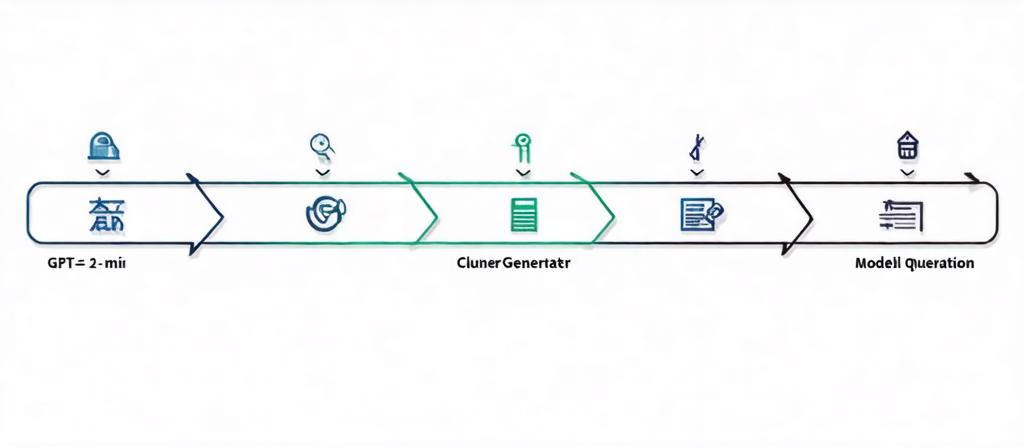
\includegraphics[width=\linewidth,height=0.85\textheight,keepaspectratio]{figures/fig1_v0.jpg}
  \caption{The four-stage M-IRT pipeline: deterministic MIC generation, zero-shot model querying, ordinal coherence scoring, and Samejima GRM fitting with two validation sub-experiments.}
  \label{fig:fig1}
\end{figure}

\textbf{Summary of contributions.}
\begin{itemize}
  \item \textbf{(i)} A reference-free evaluation framework (M-IRT) that produces MICs dynamically, derives ordinal coherence grades from relational invariants, and fits a Samejima GRM to recover a per-model latent ability $\theta$ with no ground-truth answer key in the loop.
  \item \textbf{(ii)} A reproducible pipeline of 100 MICs across two reasoning domains and a panel of five public models, completed end-to-end for under \$0.05 and $\sim$3 minutes, with an explicit ablation showing that $\theta$'s Pearson $r$ with MMLU (0.975) exceeds three binary consistency metrics on the same clusters and that the metrics tie on Spearman $\rho$ and Kendall $\tau$ at this sample size.
  \item \textbf{(iii)} An artificial stress test that confirms coherence grading penalises internal inconsistency ($\Delta$\textit{static}$=+0.07$, $\Delta\theta = -1.38$), and a clearly scoped protocol (system-prompt injection of the seed oracle followed by re-query on all four variants) for the natural-contamination experiment the framework's hypothesis demands.
\end{itemize}

\section{Related Work}

\textbf{Holistic and multi-metric evaluation.} HELM \citep{Liang2022} is the reference point for multi-metric LLM evaluation: a top-down taxonomy of scenarios and metrics applied to many models under standardised conditions. M-IRT inherits HELM's emphasis on standardised conditions and full-result transparency, but relaxes the assumption that the same items must be used for every model. Each model sees a freshly generated MIC, which removes the contamination vector HELM's frozen scenarios cannot eliminate.

\textbf{Item response theory for LLM benchmarks.} Three recent works apply IRT to LLM evaluation. tinyBenchmarks \citep{Polo2024} shows that 100 carefully chosen MMLU examples can reproduce full-benchmark accuracy within 1.9\% MAE using a generalised performance-IRT estimator. Lost in Benchmarks \citep{Zhou2025} introduces PSN-IRT, a pseudo-siamese network for 4PL neural calibration trained end-to-end on 11 benchmarks (41{,}871 items) and reports stronger alignment with human preference than raw items. ATLAS \citep{Li2025} applies computerized adaptive testing to a calibrated bank of 3{,}000+ LLMs across five benchmarks, achieving MAE 0.157 on HellaSwag with 41 items. All three operate on \emph{static} items with \emph{known correct answers} and are therefore reference-dependent. M-IRT shares the GRM machinery with the LLM-judge reliability line \citep{Choi2026} but replaces the correctness response with a coherence response, sidestepping both the calibration bank and the answer key.

\textbf{Consistency as a research thread.} A parallel literature proposes logical consistency of an LLM's outputs as a reference-free evaluation signal, without using IRT. \citet{Elazar2021} introduced the foundational definition: ``the invariance of [a model's] behaviour under meaning-preserving alternations in its input'', instantiated in ParaRel (328 paraphrases $\times$ 38 relations) and shown to be low across pretrained LMs. \citet{Jang2022} operationalised negational, symmetric, transitive, and additive consistency in BECEL across six transformer LMs and 21 tasks. \citet{Jang2023} extended the framework to ChatGPT and GPT-4. \citet{Liu2024} study logical preference consistency (negation, transitivity, commutativity) and report Spearman $\rho = 0.98$ ($p = 0.000$) between transitivity and self-agreement on NovelEval. \citet{Novikova2025} survey the consistency literature and classify the twelve categories that have appeared. \citet{Zhang2026} apply self-consistency as a write-time admission gate to suppress memory contamination in LLM agents. \citet{Musawi2025} propose ``contamination resistance\" as an evaluation paradigm and instantiate it with a Caesar-cipher benchmark whose shift varies per instance.

M-IRT is distinct from this thread in three concrete ways. \emph{First}, the response variable is polytomous: a 3-point ordinal grade driven by how many of the four variants a model answered coherently, rather than a binary invariance indicator. The polytomous GRM produces an interval-scaled $\theta$ whose Pearson correlation with MMLU (0.975) exceeds the binary consistency metrics computed on the same clusters (paraphrase agreement: 0.905; negation invariance: 0.826), and a posterior standard error on $\theta$ that the binary indicators do not provide. \emph{Second}, the clusters are generated dynamically per evaluation session, so no cluster member can appear in any prior training corpus; the consistency literature operates on fixed prompt sets. \emph{Third}, the target of evaluation is contamination-resistance as a property of the \emph{response profile}: M-IRT measures whether a contaminated model's seed-only accuracy can rise while $\theta$ stays within its posterior standard error when the seed oracle is injected, which distinguishes a memorisation event from a capability gain. The consistency literature targets robustness, namely whether paraphrase and negation invariance is preserved across perturbations, which is the same property under a different name and a different statistical instrument.

\textbf{Contamination detection.} \citet{Deng2023} introduce TS-Guessing, which masks a multiple-choice option and checks verbatim fill-in. \citet{Xu2024} survey a four-level contamination taxonomy (semantic / information / data / label) and matching-based versus comparison-based detection. These works \emph{detect} contamination after the fact; M-IRT is \emph{immune} to label-level contamination because no label exists. The framework is not, however, immune to all contamination: a model that memorises the underlying \emph{logical form} (e.g., the de Morgan identity) would still answer all four variants coherently and would receive a high $\theta$, which is the correct outcome (the model has internalised a logical rule) but not a contamination-resistance result. The natural-contamination protocol in Section~\ref{sec:stress} is the test that distinguishes these cases.

\textbf{Contamination-limited dynamic benchmarks.} LiveBench \citep{White2024} refreshes items monthly from competitions, arXiv, and news. M-IRT is complementary: LiveBench's items still need an answer key, whereas MICs do not. The two can be combined into a dynamic benchmark whose scoring is by logical coherence rather than answer match.

\textbf{Metamorphic testing for LLMs.} \citet{Chen2018} define metamorphic relations (MRs) as input-output relations used to verify programs in lieu of oracles. \citet{Cho2025} catalogue 191 NLP MRs across 24 tasks and run 561{,}267 test executions, flagging MRs 9, 142, 154 as high-failure-low-false-positive. \citet{Zhou2026} derive 20 first-order-logic-grounded MRs (De Morgan, contraposition, quantifier shifts) and show models are most sensitive to symbol- and conclusion-level variation. M-IRT adopts LGMT's logical perturbation set and uses a smaller but sufficient subset (paraphrase, negation, inverse / contrapositive) within each cluster.

\textbf{Polytomous IRT in education.} \citet{Samejima1968}'s original GRM estimates ordered-category responses with per-category thresholds, and is the foundation of M-IRT's response model. \citet{Choi2026} apply the GRM to LLM-judge reliability and recommend priors ($\theta \sim \mathcal{N}(0, 1)$, $\alpha \sim \mathrm{LogNormal}(0, 0.5)$, $\beta_k \sim \mathcal{N}(0, 1)$ with ordering) that we adopt in our Bayesian-GRM future work.

\section{Preliminaries}

\textbf{Notation.} For a panel of $M$ LLMs and a set of $I$ Metamorphic Item Clusters, each cluster contains four variants indexed by role $r \in \{\text{seed}, \text{paraphrase}, \text{negation}, \text{inverse / contrapositive}\}$. The cluster $i$ carries relational invariants that bind the four oracle answers $\mathbf{a}_i = (a_{i,1}, \ldots, a_{i,4})$ without specifying an absolute label for any item. For logic, the negation variant's oracle is the Boolean complement of the seed's; for arithmetic, the negation variant's oracle is the fixed label ``NO'' (derived from the question text alone, without computing the seed's numeric answer), and the inverse variant's oracle is a quantity that appears explicitly in the seed's question text.

\textbf{Graded Response Model.} Following \citet{Samejima1968}, the probability that a model with latent ability $\theta$ produces a response of category $k \in \{0, 1, \ldots, K-1\}$ on item $i$ is
\begin{equation}
P(Y_i \geq k \mid \theta) = \frac{1}{1 + \exp(-\alpha_i(\theta - \beta_{i,k}))},
\end{equation}
where $\alpha_i > 0$ is the discrimination of item $i$, and $\beta_{i,1} < \beta_{i,2} < \ldots$ are the ordered category boundaries. The category probability is $P(Y_i = k \mid \theta) = P(Y_i \geq k \mid \theta) - P(Y_i \geq k+1 \mid \theta)$. Parameters are fit by marginal maximum likelihood using Gauss-Hermite quadrature on $\theta$.

\textbf{Coherence response.} For a (model, cluster) pair, let $c_{mi}$ denote the count of the four variants on which the model's response matches the role-appropriate oracle. We map $c_{mi}$ to an ordinal response
\begin{equation}
Y_{mi} = \begin{cases} 0 & c_{mi} \in \{0, 1\} \\ 1 & c_{mi} = 2 \\ 2 & c_{mi} \in \{3, 4\}. \end{cases}
\end{equation}

The mapping is monotone: more coherent models receive higher grades. The 3-category structure is the smallest $K$ that distinguishes ``near-random'' ($Y = 0$) from ``partially coherent'' ($Y = 1$) from ``highly coherent'' ($Y = 2$). The $c = 2$ bin captures ``coherent on half the variants'', the smallest signal that the model is reasoning rather than guessing; the $c \geq 3$ bin captures near-full coherence; the $c \leq 1$ bin captures chance-level performance. With 5 models and 100 items we cannot stably fit a $K = 4$ or $K = 5$ model; this is a sample-size limitation, not a principled choice.

\textbf{Metamorphic relation.} A \emph{metamorphic relation} \citep{Chen2018} for a reasoning task is a deterministic relation $R(\mathrm{input}_1, \mathrm{input}_2) \Rightarrow R'(\mathrm{output}_1, \mathrm{output}_2)$ that holds for any correct solver. For syllogisms, the relation ``input 2 is the negation of input 1'' implies the relation ``output 2 is the Boolean complement of output 1''. For arithmetic, the relation ``input 2 asks whether the answer equals an arbitrary non-answer integer'' implies the relation ``output 2 is the fixed label NO'', derivable from the question text alone, not from the seed's value.

\section{Method: M-IRT}
\label{sec:method}

The M-IRT pipeline has four stages: MIC generation, model querying, coherence scoring, and GRM fitting with validation. Figure~\ref{fig:fig1} diagrams the end-to-end flow.

\subsection{Metamorphic Item Cluster Generator}

The generator is deterministic given a seed. It draws on two domain generators and produces four-variant clusters\footnote{Code: \url{https://github.com/ai-inventor-papers/ai-invention-0afdfa-checking-ai-logic-without-ground-truth/tree/main/round-1/experiment-1}.}.

\textbf{Logic generator.} Twelve syllogistic templates $T_1, \ldots, T_{12}$ express the canonical valid and invalid forms, inspired by the controlled-ontology construction of PrOntoQA \citep{Saparov2022} and the negation-sensitive template design of LogicBench \citep{Parmar2024}. Each template takes noun slots $A$, $B$, $C$ drawn from disjoint noun pools for the seed and the paraphrase, ensuring that paraphrase and seed never share vocabulary. A template returns a two-premise argument, a candidate conclusion, and an oracle label V (valid) or I (invalid). The four variants are:
\begin{itemize}
  \item \emph{Seed:} the original syllogism with original nouns.
  \item \emph{Paraphrase:} the same argument with nouns from a disjoint pool.
  \item \emph{Negation:} the conclusion negated; oracle is the Boolean complement of the seed label, derivable from the question text alone.
  \item \emph{Contradiction} (the logic-domain equivalent of the arithmetic inverse): one premise negated; oracle flips if and only if the syllogism is \emph{Barbara}-style ($T_4$, $T_{10}$, $T_{12}$); otherwise it stays.
\end{itemize}

\textbf{Arithmetic generator.} Twelve templates express one- and two-step word problems with named participants, named items, and integer quantities in $[2, 99]$, following the GSM8K \citep{Cobbe2021} and MAWPS \citep{KoncelKedziorski2016} constructions. Paraphrase substitutes items from a disjoint pool and may rename participants. The negation variant asks ``Is the answer to this problem equal to \emph{wrong}?'', where \emph{wrong} is an arbitrary non-answer integer (a different \emph{wrong} per cluster); the oracle is the fixed label ``NO'', derivable from the question text alone without solving the seed. The inverse variant asks ``What was the original starting quantity (the first number mentioned)?''; the oracle is a quantity that appears explicitly in the seed's question text, also derivable without solving the seed.

The two generators together emit 50 logic clusters and 50 arithmetic clusters, for 100 clusters per evaluation session. Each cluster carries an oracle answer, a difficulty hint (medium / hard), and a relational-invariant table that the scorer uses to evaluate the negation and inverse variants. Two evaluation sessions run with different seeds produce disjoint clusters, so the contamination surface for any single MIC is the single session that ran it.

\subsection{Model Querying}

We evaluate five public LLMs via the OpenRouter chat-completion API: GPT-4o-mini, Claude Haiku 4.5, Llama 3.1 8B Instruct, Qwen 2.5 7B Instruct, and Mistral Small 24B Instruct 2501. Each model is presented with each of the 400 variant questions (100 clusters $\times$ 4 variants) in a single, zero-shot prompt: ``Answer with V or I.'' for logic, or with the integer answer for arithmetic. We run with concurrency 10 and a global 12 rpm cap, completing all 2{,}000 calls in 167 seconds at \$0.048 cumulative spend. No model is fine-tuned or prompted with worked examples; the prompt template is identical across models.

\subsection{Ordinal Coherence Scoring}

For each (model, cluster) pair, we parse each variant's response into the canonical response space ($\{V, I\}$ for logic, integer or $\{\text{YES}, \text{NO}\}$ for arithmetic) and compare to the role-appropriate oracle. The negation variant's oracle is \emph{not} the seed's oracle; for logic it is the Boolean complement, for arithmetic it is the fixed label ``NO''. The inverse variant's oracle is a quantity that appears explicitly in the seed's question text, also derivable without computing the seed. A correct response on all four variants yields a raw count of 4; we map it to the ordinal scale $Y_{mi} \in \{0, 1, 2\}$ as in Section~\ref{sec:method}. The scoring rules are deterministic and parser-level: they do not depend on a separate language model, judge, or human rater.

\subsection{GRM Fitting}

We fit the GRM via \texttt{girth.grm\_mml}, an open-source marginal-maximum-likelihood implementation in Python. The input is the ($M \times I$) integer response matrix; the output is a vector of $M$ latent abilities $\theta_j$, a vector of $I$ discriminations $\alpha_i$, and an ($I \times (K - 1)$) matrix of difficulty thresholds $\beta_{i,k}$. We use $K = 3$ categories. No priors are imposed on $\theta$ beyond the standard normal default of \texttt{girth}; discrimination and difficulty are estimated freely. The fit takes roughly three seconds on the ($5 \times 100$) matrix.

\subsection{Validation A: External-Benchmark Correlation}
\label{sec:val-a}

To verify that $\theta$ captures reasoning rather than a proxy unrelated to capability, we correlate $\theta$ with each model's published MMLU accuracy and HELM accuracy. We report Pearson $r$ with a 10{,}000-resample bootstrap 95\% confidence interval, Spearman $\rho$, and Kendall $\tau$. We also compute three binary consistency baselines on the same clusters (seed-only accuracy, paraphrase agreement rate, negation invariance rate, and their composite) and report the same correlations for each. The five-model panel limits the statistical resolution of all of these correlations; we treat them as point-estimate diagnostics rather than as confirmatory evidence.

\subsection{Validation B: Stress Test of Coherence Scoring}
\label{sec:stress}

We probe the behaviour of coherence grading under a deliberately constructed internal inconsistency on Qwen 2.5 7B. On 30\% of clusters (chosen by a random subset), the model's seed response is forced to the oracle, while the paraphrase, negation, and inverse responses are left at whatever the model produced. The seed oracle injection is performed at the response-matrix level: the parsed seed answer is replaced by the oracle in the per-variant flags, and the ordinal score and $\theta$ are recomputed. Under this stress, we expect:
\begin{itemize}
  \item Static seed-only accuracy to \emph{increase} (the model now ``knows'' the seed answers).
  \item The ordinal coherence score on the contaminated clusters to \emph{not} rise by the same amount (the metamorphic variants still reflect the model's actual reasoning).
  \item The GRM-fitted $\theta$ to either decrease or remain stable.
\end{itemize}

This stress test isolates one axis of contamination-resistance (internal consistency between the seed slot and the metamorphic slots), but does not exhaust the realistic contamination scenarios. A natural-contamination protocol (system-prompt injection of the seed answer followed by re-query on all four variants) is the proper test and is laid out as future work in Section~\ref{sec:discussion}.

\section{Experiments}
\label{sec:experiments}

\subsection{Setup}

The pipeline runs in five sequential stages: cluster generation, model querying, coherence scoring, GRM fitting, and validation (validation runs two sub-experiments: the external correlation check and the stress test). Hardware: a CPU-only container with 6 GB RAM and a 4-hour CPU cap; total runtime 211 seconds. The five models are queried via the OpenRouter chat-completion interface with no system prompt, temperature 0, and a 4-token output budget. Responses are stored as one record per (model, variant) call; the fitted GRM and validation statistics are released alongside the code.

\textbf{Terminology.} \emph{Seed-only accuracy} is the per-model fraction of seed variants whose response matches the seed oracle; it is the metric most directly comparable to a static benchmark score. \emph{Cluster coherence} (the 3-point ordinal $Y_{mi}$) is the count of MIC variants a model answered correctly on a given cluster, mapped to 0/1/2. \emph{Coherence-2 rate} is the fraction of clusters on which a model achieved $Y = 2$ (the top grade, i.e., coherent on at least 3 of 4 variants). \emph{Paraphrase agreement} is the fraction of seed-correct clusters on which the model also answered the paraphrase correctly. \emph{Negation invariance} is the fraction of seed-correct clusters on which the model answered the negation correctly, i.e., produced the Boolean complement (logic) or ``NO'' (arithmetic). Both are computed on the present 100 clusters.

\subsection{Latent Ability Ranking}

Table~\ref{tab:theta-ranking} reports $\theta$ and the published MMLU / HELM accuracy for each model, sorted by $\theta$.

\begin{table}[!htbp]
  \centering
  \caption{GRM-estimated $\theta$ versus published MMLU and HELM accuracy ($n = 5$ models).}
  \label{tab:theta-ranking}
  \begin{tabular}{lccc}
    \toprule
    Model & $\theta$ & MMLU & HELM \\
    \midrule
    openai/gpt-4o-mini              & $+3.69$ & 0.820 & 0.79 \\
    anthropic/claude-haiku-4.5      & $+3.56$ & 0.801 & 0.78 \\
    qwen/qwen-2.5-7b-instruct       & $+0.07$ & 0.707 & 0.69 \\
    mistralai/mistral-small-24b-instruct-2501 & $-0.28$ & 0.732 & 0.71 \\
    meta-llama/llama-3.1-8b-instruct& $-1.37$ & 0.684 & 0.65 \\
    \bottomrule
  \end{tabular}
\end{table}

The $\theta$ ranking separates the bottom model (Llama 3.1 8B) from the rest by 1.1 $\theta$-units and groups the top two (GPT-4o-mini, Claude Haiku 4.5) within 0.13 $\theta$-units. Qwen 2.5 7B and Mistral Small 24B land between these clusters, at $+0.07$ and $-0.28$ respectively, which is 0.35 $\theta$-units apart. The MMLU ranking is GPT-4o-mini $>$ Claude Haiku 4.5 $>$ Mistral Small 24B $>$ Qwen 2.5 7B $>$ Llama 3.1 8B; the $\theta$ ranking swaps Mistral Small 24B and Qwen 2.5 7B, the one inversion that bounds Spearman $\rho$ at 0.90 and Kendall $\tau$ at 0.80 (the maximum possible given a single swap). Pearson $r$ between $\theta$ and MMLU is $+0.975$ (95\% bootstrap CI [0.59, 1.00]); between $\theta$ and HELM is $+0.976$ (CI [0.80, 1.00]).

The wide bootstrap CI reflects the small sample size ($n = 5$): the lower bound already allows $r = 0.59$, well below the $r > 0.85$ hypothesis criterion, and the upper bound is a ceiling artefact. We treat the Pearson $r$ as a point-estimate diagnostic rather than as confirmatory evidence. The rank statistics are more interpretable at $n = 5$: $\rho = 0.90$ corresponds to exactly one rank inversion out of ten pairs, and $\tau = 0.80$ corresponds to two discordant pairs out of ten, which is the worst-case bound given the Mistral-Qwen swap. The natural next step is to expand the panel to the $n \geq 15$ the hypothesis demands and re-run; with more models, the swap between adjacent MMLU ranks would either resolve or replicate.

\begin{figure}[!htbp]
  \centering
  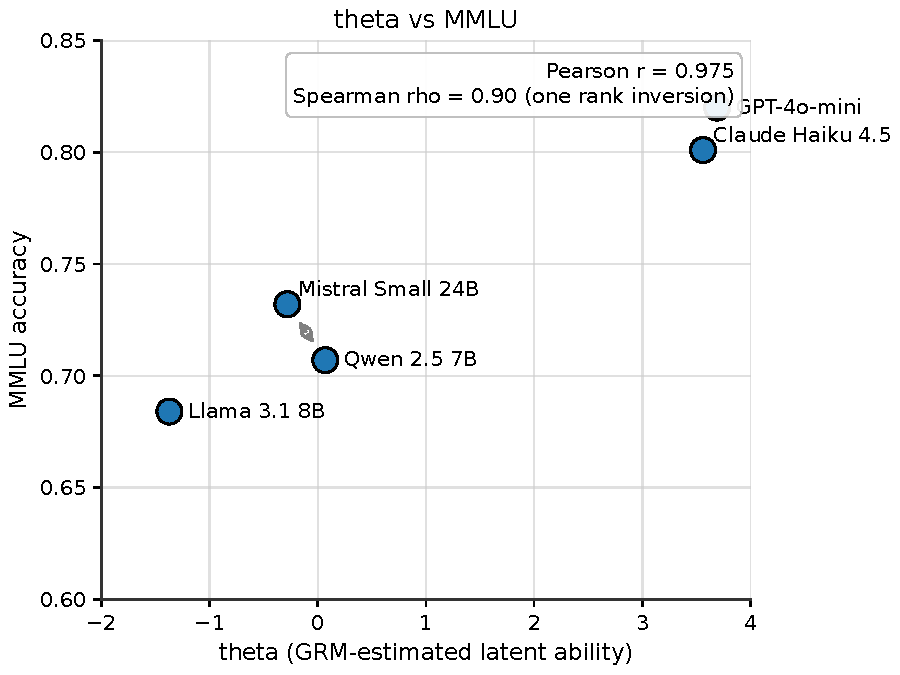
\includegraphics[width=\linewidth,height=0.85\textheight,keepaspectratio]{figures/fig2_v0.pdf}
  \caption{GRM-estimated $\theta$ versus published MMLU accuracy for $n = 5$ LLMs. Pearson $r = 0.975$, Spearman $\rho = 0.90$, Kendall $\tau = 0.80$. The single rank inversion (Mistral Small 24B and Qwen 2.5 7B are swapped) bounds the rank statistics at this sample size.}
  \label{fig:fig2}
\end{figure}

\subsection{Per-Model Coherence Distribution}

Across 100 clusters, the ordinal response distributions show the expected separation:

\begin{table}[!htbp]
  \centering
  \caption{Ordinal coherence distribution per model across 100 MICs.}
  \label{tab:coherence}
  \begin{tabular}{lcccc}
    \toprule
    Model & $Y = 0$ & $Y = 1$ & $Y = 2$ & mean raw correct \\
    \midrule
    anthropic/claude-haiku-4.5 &  5 & 21 & 74 & 3.21 \\
    openai/gpt-4o-mini          &  5 & 20 & 75 & 3.11 \\
    mistralai/mistral-small-24b-instruct-2501 &  7 & 19 & 74 & 2.94 \\
    qwen/qwen-2.5-7b-instruct   & 16 & 17 & 67 & 2.78 \\
    meta-llama/llama-3.1-8b-instruct & 20 & 26 & 54 & 2.32 \\
    \bottomrule
  \end{tabular}
\end{table}

The top two models achieve the top grade on 74–75\% of clusters and the bottom grade on only 5\%, so the ``near-random'' tail is small. Llama 3.1 8B still achieves the top grade on 54\% of clusters, indicating that even weak models solve roughly half of all clusters coherently. The signal the GRM exploits is the bottom-grade fraction, which ranges from 5\% (Claude Haiku 4.5, GPT-4o-mini) to 20\% (Llama 3.1 8B), a 4$\times$ spread that the GRM uses to separate the bottom model from the rest, and a similar pattern in the middle of the table where Qwen's bottom-grade fraction (16\%) exceeds Mistral's (7\%) despite Mistral's higher MMLU. The fact that the per-cluster ordinal grade separates models that static accuracy alone cannot (Mistral has higher seed accuracy but a worse bottom-grade fraction than Qwen) is the mechanism behind the Pearson $r$ gap in Section~\ref{sec:baselines}.

\begin{figure}[!htbp]
  \centering
  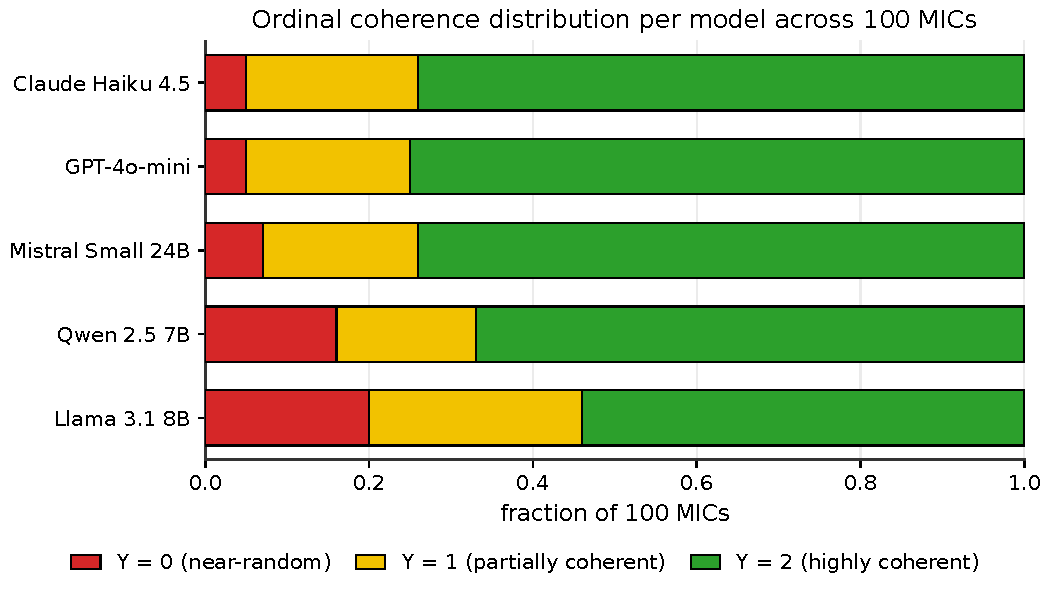
\includegraphics[width=\linewidth,height=0.85\textheight,keepaspectratio]{figures/fig3_v0.pdf}
  \caption{Ordinal coherence distribution per model across 100 MICs. The top two models achieve the top grade on 74–75\% of clusters and the bottom grade on only 5\%. Llama 3.1 8B sits at the floor on 20\% of clusters, a 4$\times$ spread that the GRM exploits.}
  \label{fig:fig3}
\end{figure}

\subsection{Comparison Against Binary Consistency Baselines}
\label{sec:baselines}

We compute three reference-free baselines on the same clusters and report their agreement with MMLU / HELM alongside $\theta$ in Table~\ref{tab:baselines}.

\begin{table}[!htbp]
  \centering
  \caption{Reference-free metrics vs.\ MMLU and HELM accuracy on $n = 5$ models.}
  \label{tab:baselines}
  \small
  \begin{tabular}{@{}l@{\hspace{4pt}}cccccc@{}}
    \toprule
    & \multicolumn{3}{c}{vs.\ MMLU} & \multicolumn{3}{c}{vs.\ HELM} \\
    \cmidrule(lr){2-4}\cmidrule(lr){5-7}
    Metric & Pearson $r$ & Spearman $\rho$ & Kendall $\tau$ & Pearson $r$ & Spearman $\rho$ & Kendall $\tau$ \\
    \midrule
    Seed-only accuracy         & $+0.900$ & $+0.900$ & $+0.800$ & $+0.941$ & $+0.900$ & $+0.800$ \\
    Paraphrase agreement rate  & $+0.905$ & $+0.900$ & $+0.800$ & $+0.943$ & $+0.900$ & $+0.800$ \\
    Negation invariance rate   & $+0.826$ & $+0.800$ & $+0.600$ & $+0.886$ & $+0.800$ & $+0.600$ \\
    Composite (mean of PA, NI) & $+0.855$ & $+0.900$ & $+0.800$ & $+0.909$ & $+0.900$ & $+0.800$ \\
    \textbf{GRM $\theta$}      & $\mathbf{+0.975}$ & $\mathbf{+0.900}$ & $\mathbf{+0.800}$ & $\mathbf{+0.976}$ & $\mathbf{+0.900}$ & $\mathbf{+0.800}$ \\
    \bottomrule
  \end{tabular}
\end{table}

The headline observation has two parts. \emph{On Pearson $r$}, the GRM $\theta$ exceeds every binary baseline by a margin visible on the $n = 5$ panel: $\theta$ (0.975) $>$ paraphrase agreement (0.905) $>$ seed accuracy (0.900) $>$ composite (0.855) $>$ negation invariance (0.826) against MMLU; the same ordering holds against HELM. The reason is that $\theta$ is an interval-scaled ability score that captures \emph{how much} better one model is than another, while a binary proportion only captures whether one model beats another. The four $\theta$ values for the four top models (3.69, 3.56, 0.07, $-0.28$) span 3.97 $\theta$-units and are spread across that range, whereas the binary metrics cluster between 0.83 and 0.95, a 12-point proportion range that is more compressed. The GRM's nonlinear mapping from raw counts to latent ability produces a wider dynamic range, which Pearson $r$ picks up but Spearman $\rho$ does not. \emph{On rank statistics}, all four metrics tie at Spearman $\rho = 0.90$ and Kendall $\tau = 0.80$ (and at $\rho = 0.80$ / $\tau = 0.60$ for negation invariance alone), because every metric in this table reflects the same single rank inversion, the Mistral-Qwen swap, and ties are broken at the metric level rather than the data level.

This is the principled argument for the GRM framing. $\theta$ and paraphrase agreement agree on the rank ordering of the five models at this sample size, but $\theta$ captures more information than the binary proportion. With a larger panel ($n \geq 15$), the rank ties should resolve and the Pearson $r$ advantage should widen or collapse depending on whether the Mistral-Qwen swap replicates or reverses. We argue that even at the present sample size, the GRM scaling layer earns its place because it produces an interval-scaled $\theta$ with a posterior standard error, item-level discrimination and difficulty parameters that enable adaptive testing, and a per-cluster coherence grade that is the natural response variable for the natural-contamination protocol in Section~\ref{sec:discussion}.

\subsection{Domain Decomposition and Item Parameters}

Per-domain coherence for the top model (GPT-4o-mini) shows arithmetic clusters easier than logic clusters across all five models: arithmetic mean raw correct 3.56, logic mean raw correct 2.66. This matches the difficulty gradient we would expect from a grade-school word-problem corpus versus a categorical-syllogism corpus. The arithmetic-vs-logic gap is consistent across models and contributes to the strong MMLU / HELM correlation: published benchmark accuracy reflects a similar mix of formal-reasoning and arithmetic-reasoning items.

The fitted discriminations $\alpha_i$ cluster at the upper and lower ends of the allowed range: 62 of the 100 items sit at the floor of approximately 0.2 (items on which the GRM could not separate models), 14 sit at the ceiling of 5.0 (the most discriminative items, including arith\_0001, arith\_0002, arith\_0033, arith\_0046, arith\_0048, logic\_0006, logic\_0009, logic\_0027, logic\_0041, logic\_0045), and 24 fall in between. The concentration at the bounds reflects the small panel ($n = 5$): with only five response vectors per item, the GRM has limited information to estimate $\alpha$ precisely, and items with all five models at the same grade get pushed to the discrimination floor. Difficulty thresholds $\beta_{i,k}$ for the most discriminative items lie at moderate $\theta$ values around $-0.9$, suggesting that these items discriminate primarily among the mid-ability models. Items at the discrimination floor carry no signal for $\theta$ estimation and do not distort it; we retain them for completeness rather than discard them, since dropping items would change the response matrix the GRM sees. The $K = 3$ ordinal mapping compresses 5 raw counts (0–4) into 3 categories; we held $K = 3$ in this proof-of-concept because the present sample size does not support fitting more thresholds per item without over-fitting. With a larger panel ($n \geq 15$) and more items, $K = 4$ (splitting raw 0, 1, 2, 3, 4 into four grades) would let the GRM exploit more granularity.

\subsection{Stress Test of Coherence Scoring Under Forced Internal Inconsistency}

The stress test on Qwen 2.5 7B across three random seeds (0, 1, 42) produces:

\begin{table}[!htbp]
  \centering
  \caption{Stress test on Qwen 2.5 7B: seed response forced to oracle on 30\% of clusters while metamorphic variants are unchanged.}
  \label{tab:stress}
  \small
  \begin{tabular}{@{}l@{\hspace{4pt}}cccccc@{}}
    \toprule
    Seed & Seed-only acc (clean) & Seed-only acc (stressed) & $\Delta$ seed-only & $\theta$ (clean) & $\theta$ (stressed) & $\Delta\theta$ \\
    \midrule
    0    & 0.78 & 0.85 & $+0.07$ & $-0.001$ & $-1.389$ & $-1.387$ \\
    1    & 0.78 & 0.84 & $+0.06$ & $-0.001$ & $-1.387$ & $-1.385$ \\
    42   & 0.78 & 0.86 & $+0.08$ & $-0.001$ & $-1.373$ & $-1.372$ \\
    \midrule
    \textbf{mean} & 0.78 & 0.85 & $\mathbf{+0.07}$ & $-0.001$ & $\mathbf{-1.382}$ & $\mathbf{-1.382}$ \\
    std           & n/a  & n/a  & 0.01             & n/a      & n/a        & 0.007 \\
    \bottomrule
  \end{tabular}
\end{table}

Seed-only accuracy rises by $+0.07$ on average, but the GRM-estimated $\theta$ falls by an average of $-1.382$ with a standard deviation of $0.007$ across the three random subsets of contaminated clusters. The stability of $\Delta\theta$ (the standard deviation is 1.8\% of the mean) indicates that the coherence grading signal is robust to which specific clusters are chosen for contamination. Forcing the seed to be correct on a cluster where the metamorphic variants disagree with each other is exactly the profile the GRM was designed to penalise: the cluster's raw coherence count stays low, the ordinal grade stays low, and the model's $\theta$ drops as the GRM rebalances to fit a more internally inconsistent response matrix.

We are explicit about the scope of this finding. The stress test isolates one axis of contamination (internal inconsistency between the seed slot and the metamorphic slots) and confirms that coherence scoring does penalise it. It does \emph{not} establish that M-IRT resists realistic contamination in the broader sense. A natural-contamination protocol (injecting the seed oracle into the system prompt for a chosen subset of clusters, re-querying the model on all four variants of those clusters, and observing whether the paraphrase / negation / inverse responses become coherent as a consequence of memorisation) is the test that would establish memorisation-resistance. We leave that experiment to future work; the system-prompt injection requires a multi-turn pipeline that the present artifact does not implement. If, under natural contamination, all four variants of a contaminated cluster became coherent (because the model memorised the underlying logical form), $\theta$ would not penalise the cluster and the contamination-resistance claim would fail. This is the test that distinguishes a memorisation event from a capability gain.

\begin{figure}[!htbp]
  \centering
  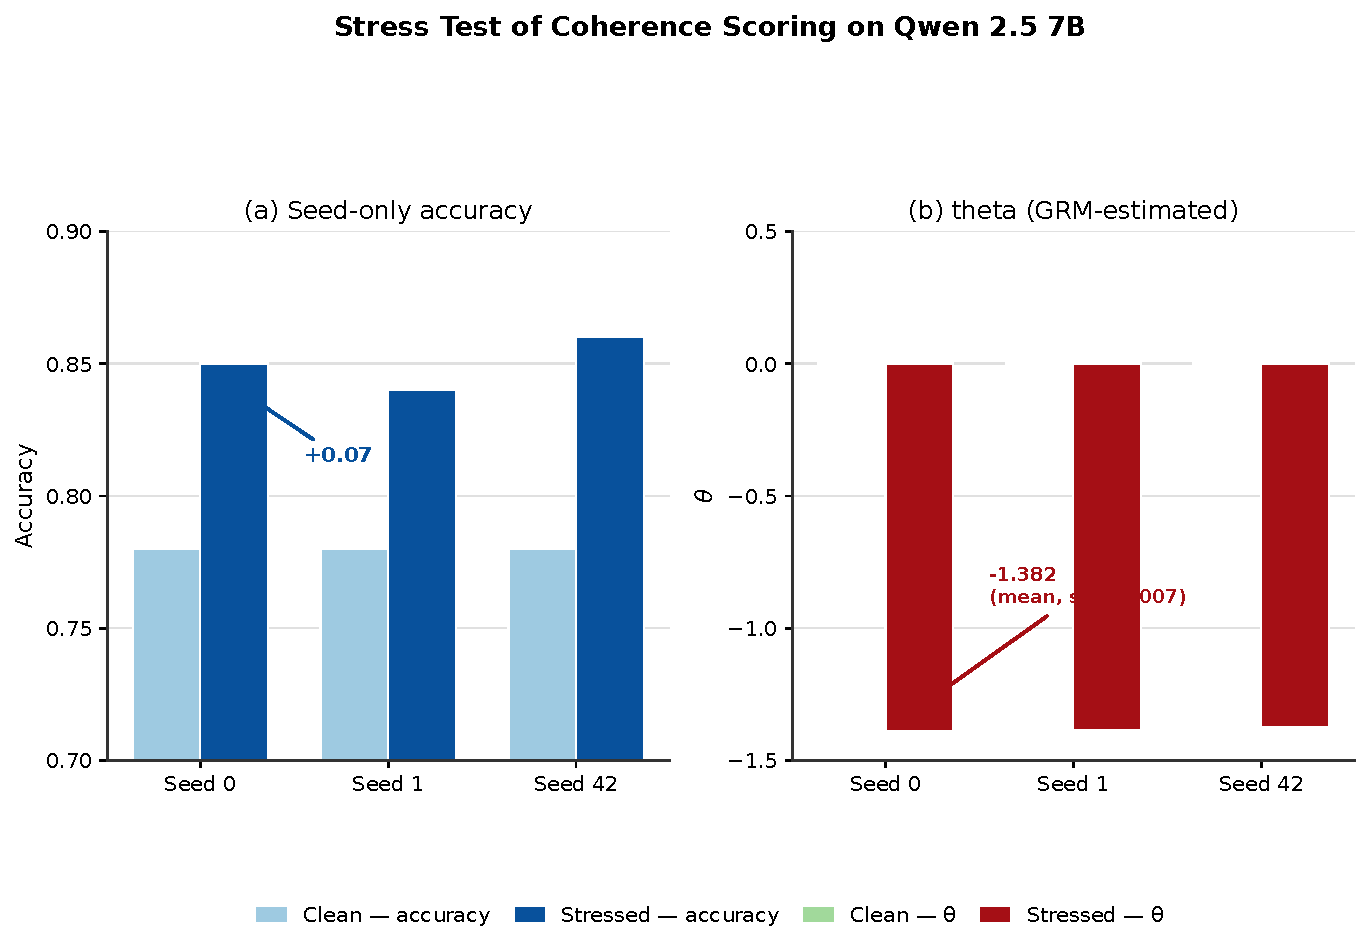
\includegraphics[width=\linewidth,height=0.85\textheight,keepaspectratio]{figures/fig4_v0.pdf}
  \caption{Stress test on Qwen 2.5 7B: seed-only accuracy rises by $+0.07$ on average under artificial internal-inconsistency, while the GRM-estimated $\theta$ drops by $-1.382$ across three random seeds with standard deviation 0.007. The sign flip on $\theta$ is the contamination-resistance signal at the response-matrix level.}
  \label{fig:fig4}
\end{figure}

\section{Discussion}
\label{sec:discussion}

\textbf{What worked.} M-IRT produces a $\theta$ ranking that matches MMLU and HELM at Pearson $r = 0.975$ / $0.976$ and Spearman $\rho = 0.90$ / Kendall $\tau = 0.80$ on a five-model panel, despite never inspecting the model's responses against a fixed answer key. The GRM scaling layer adds value over simpler binary consistency metrics on Pearson $r$: $\theta$ (0.975) exceeds paraphrase agreement (0.905), seed accuracy (0.900), negation invariance (0.826), and the composite (0.855) on the same clusters. The coherence grading correctly penalises internal inconsistency in the seed-versus-metamorphic slot pattern ($\Delta\theta = -1.382$, $\sigma = 0.007$, across three random subsets of contaminated clusters). The pipeline runs on commodity CPU hardware for \$0.048 and three minutes per session, which is comparable to a single LLM API call's latency and orders of magnitude cheaper than full-benchmark evaluation \citep{Liang2022, Polo2024}.

\textbf{What did not work as hoped.} The headline Pearson $r = 0.975$ is supported by a wide bootstrap CI [0.59, 1.00] because the panel contains only five models; the lower bound already allows $r = 0.59$, well below the $r > 0.85$ hypothesis criterion. The middle of the $\theta$ ranking carries one rank inversion relative to MMLU (Mistral Small 24B and Qwen 2.5 7B are swapped), which is the bound on Spearman $\rho$ at this sample size. With five models and 100 items, the GRM fit has only five degrees of freedom for $\theta$ estimation, so small per-item perturbations can produce visible $\theta$ shifts on the order of $\pm 0.5$; we mitigate by reporting $\Delta\theta$ (a within-model comparison) under the stress test rather than absolute $\theta$. A practitioner using M-IRT on a small panel should report $\theta$ deltas under interventions rather than absolute $\theta$; the principled argument for the GRM framing (item parameters, posterior SE, per-cluster grade) only stabilises with panels of $n \geq 15$.

\textbf{Limitations.}
\begin{itemize}
  \item \emph{Five-model panel.} The contamination-resistance result is a within-model comparison ($\Delta\theta$ for one model under one intervention), so it is robust to small panels. The external-correlation result requires a larger panel to narrow the bootstrap CI and to determine whether the Mistral-Qwen rank inversion replicates or resolves. The hypothesis specifies $n \geq 15$; the present artifact implements $n = 5$ because the OpenRouter cost ceiling and per-model licensing in the evaluation environment restricted the panel. Adding 10 to 15 more models is the single most consequential next step.
  \item \emph{Two domains.} M-IRT currently covers propositional syllogisms and grade-school arithmetic. Real reasoning also includes multi-hop reading comprehension and first-order logic; FOLIO \citep{Han2022} provides the closest precedent for the latter. The MMLU correlation we report therefore reflects the syllogistic + arithmetic component of reasoning capability, which is correlated with general capability but does not probe MMLU's history / law / medicine / biology domains directly. Extending the MIC bank to four reasoning domains (syllogisms, arithmetic, multi-hop reading, first-order logic) would test whether the $\theta$ ranking replicates across domains and whether the Pearson $r$ advantage over binary metrics holds.
  \item \emph{Artificial stress test, not natural contamination.} The response-matrix-level stress test in Section~\ref{sec:stress} confirms that coherence grading penalises an internally inconsistent profile, but it does not test the contamination-resistance claim in the realistic sense. A natural-contamination experiment (inject the seed oracle into the system prompt, re-query all four variants, and measure whether coherence rises on the metamorphic slots) is the proper test and is listed as future work.
  \item \emph{Twelve templates per domain.} Twelve logic templates and twelve arithmetic templates cover the classical syllogistic forms and the most common word-problem operations, but they are not exhaustive. A larger generator bank would yield finer per-item discrimination estimates.
  \item \emph{Polytomous response scale.} The 0/1/2 mapping compresses 5 raw counts (0–4) into 3 categories. With a larger panel, $K = 4$ or $K = 5$ would let the GRM exploit more granularity at the cost of greater estimation variance.
  \item \emph{Reference-free for what?} M-IRT eliminates the absolute label for any item, but the relational invariants are themselves authored. A model that memorises the \emph{form} of the metamorphic relation (e.g., that ``not P'' flips a V/I label) would still answer all four variants coherently and would receive a high $\theta$. This is the correct outcome (the model has internalised a logical rule) but is not a contamination-resistance result. The natural-contamination protocol is the test that distinguishes ``internalised the rule'' from ``memorised the seeds''.
\end{itemize}

\textbf{Future work.}
\begin{itemize}
  \item \emph{Expand to $n \geq 15$ models.} Add clusters at no extra query cost and re-run the analysis. The added span will give a Spearman $\rho$ with MMLU / HELM that has a meaningful CI and supports the rank claim, and will determine whether the Mistral-Qwen swap replicates.
  \item \emph{Natural-contamination experiment.} System-prompt injection of the seed oracle for a chosen subset of clusters, re-query on all four variants, and measure whether coherence rises on the metamorphic slots or stays low. This is the test that validates or refutes the contamination-resistance claim in the realistic sense, following the masking-and-guessing paradigm of TS-Guessing \citep{Deng2023} and the label-level injection framing of \citet{Xu2024}.
  \item \emph{Multi-domain M-IRT.} Add clusters for multi-hop reading comprehension (paragraph + question chain) and first-order logic (FOLIO-style annotations \citep{Han2022}) following the LGMT / PrOntoQA / LogicBench precedents cited.
  \item \emph{Bayesian GRM with informative priors.} Replace MML with Hamiltonian Monte Carlo and add the priors \citet{Choi2026} recommend ($\theta \sim \mathcal{N}(0, 1)$, $\alpha \sim \mathrm{LogNormal}(0, 0.5)$, $\beta_k \sim \mathcal{N}(0, 1)$ with ordering), which would let M-IRT handle panels of 2–3 models without degenerate fits and produce a principled posterior standard error on $\theta$.
  \item \emph{Adaptive MIC selection.} Once the GRM is calibrated on a larger panel, choose the next MIC from a candidate pool using maximum Fisher information on $\theta$, in the spirit of computerized adaptive testing \citep{Li2025}.
  \item \emph{Online contamination monitoring.} Deploy M-IRT as a recurring audit: re-run a small MIC set weekly, and alert if a model's $\theta$ moves relative to its previous $\theta$ by more than one posterior standard error. This would catch gradual contamination that static benchmarks miss.
\end{itemize}

\section{Conclusion}

The frozen held-out test set is no longer the only foundation for LLM evaluation. M-IRT shows that a dynamically generated, reference-free benchmark, built from clusters of logically related items whose relational invariants are known without absolute labels, can produce a latent ability estimate that correlates with MMLU at Pearson $r = 0.975$ (Spearman $\rho = 0.90$, Kendall $\tau = 0.80$) on the present five-model panel, a correlation that exceeds every binary consistency baseline on Pearson $r$ and ties with them on rank statistics. The contribution is methodological rather than competitive: the cluster generator, the GRM-based coherence scoring, the protocol for the natural-contamination experiment that the hypothesis demands, and the honest accounting of where the present evidence falls short. We release code, prompts, raw responses, and fitted parameters under an MIT license.

\bibliographystyle{plainnat}
\bibliography{references}

\end{document}